\chapter{适定问题}

\section{预备知识}

通常只考虑对适定问题的数值求解,这一章明确什么样的问题是适定的。
我们考虑的问题默认都是纯初值问题,定义域为整个空间,并且在空间上的每一个维度都具有 $2\pi$ 周期,从而可以在分析时使用Fourier方法,考虑谐波解。

\begin{definition}
    称问题是适定的,若存在唯一解,并且解关于初值是稳定的,即:存在常数 $K,\alpha>0$,使得
    \[
        \| u(x,t) \| \le Ke^{\alpha(t-t_0)} \| u(x,t_0) \|
    \]
\end{definition}

基本的例子:
\begin{enumerate}
    \item 对流方程 $u_t + a u_x = 0$ 对于任意 $a \in \mathbb{R}$ 都是适定的;
          \begin{gather*}
              \frac12 \frac{d}{dt} \| u \|^2 = \int_{0}^{2\pi} u u_t \,dx = - a \int_0^{2\pi} u u_x\,dx
              = - \frac{a}2 u^2\big|_0^{2\pi} = 0
              \\
              \Rightarrow \quad \| u(x,t) \|^2 = \| u(x,0) \|^2
          \end{gather*}
    \item 扩散方程 $u_t = b u_{xx}$ 对于 $b > 0$ 是适定的,但是 $b < 0$ 是不适定的;
          \begin{gather*}
              \frac12 \frac{d}{dt} \| u \|^2 = \int_{0}^{2\pi} u u_t \,dx = b \int_0^{2\pi} u u_{xx}\,dx
              = b u u_x \big|_0^{2\pi} - b \int_{0}^{2\pi} (u_x)^2\,dx = - b \int_{0}^{2\pi} (u_x)^2\,dx \le 0
              \\
              \Rightarrow \quad \| u(x,t) \|^2 \le \| u(x,0) \|^2, \quad (b > 0)
          \end{gather*}
\end{enumerate}
对于含低阶项的方程也可以分析,例如
\[
    u_t = u_x + \alpha\,u, \quad (\alpha \in \mathbb{R})
\]
进行变量代换,定义 $v = e^{-\alpha t} u$,可以得到 $v$ 满足的方程
\[
    \left\{
    \begin{aligned}
        v_t & = e^{-\alpha t} (u_t - \alpha u), \\
        v_x & = e^{-\alpha t} u_x
    \end{aligned}
    \right.
    \quad \Rightarrow \quad v_t = v_x
\]
由于换元之后的方程是适定的,因此原方程也是适定的。
\[
    \| v(x,t) \|^2 = \| v(x,0) \|^2, \quad \Rightarrow \quad \| u(x,t) \|^2 = e^{2 \alpha t} \| u(x,0) \|^2.
\]

对于方程组问题,例如对称双曲方程组
\[
    U_t = A\,U_x =
    \begin{bmatrix}
        0 & d \\
        d & 0
    \end{bmatrix}
    U_x,
\]
对 $A$ 可以进行正交相似对角化
\[
    A = R \Lambda R^\mathsf{H},\quad
    R = \frac{1}{\sqrt{2}}
    \begin{bmatrix}
        -1 & 1 \\
        1  & 1
    \end{bmatrix},\quad
    \Lambda =
    \begin{bmatrix}
        -d & 0 \\
        0  & d
    \end{bmatrix}
\]
换元 $W  = R^\mathsf{H} U$,可以得到 $W$ 满足
\[
    W_t = \Lambda\,W_x =
    \begin{bmatrix}
        -d & 0 \\
        0  & d
    \end{bmatrix}
    W_x,
\]
因此原问题是适定的。
再例如考虑非对称双曲方程组
\[
    U_t = B\,U_x =
    \begin{bmatrix}
        0   & 1 \\
        d^2 & 0
    \end{bmatrix}
    U_x
\]
通过相似变换
\[
    B = D S D^{-1},\quad
    D =
    \begin{bmatrix}
        1 & 0 \\
        0 & d
    \end{bmatrix},\quad
    S =
    \begin{bmatrix}
        0 & d \\
        d & 0
    \end{bmatrix}
\]
换元 $V = D^{-1} U$,可以得到 $V$ 满足
\[
    V_t = S\,V_x =
    \begin{bmatrix}
        0 & d \\
        d & 0
    \end{bmatrix}
    V_x
\]
回到了对称双曲方程组的情形,因此原问题也是适定的。

\section{一维常系数标量方程的适定性}

考虑一维常系数标量方程:周期函数 $u: \mathbb{R} \times \mathbb{R}^+ \to \mathbb{C}$,
常系数 $a,b,c \in \mathbb{C}$,满足的 PDE 为
\begin{equation}
    \left\{
    \begin{aligned}
         & u_t = a u_{xx} + b u_x + c u, \\
         & u(x,0) = f(x)
    \end{aligned}
    \right.
    \label{eq:1d-pde-scalar}
\end{equation}
谐波解形如
\[
    \hat{u}(\omega,t) = e^{\kappa t} \hat{f}(\omega), \quad  \kappa := -a \omega ^2 + i b \omega  + c.
\]

\begin{theorem}\label{thm:well-posed-1}
    问题~\eqref{eq:1d-pde-scalar} 是适定的,等价于存在常数 $\alpha \in \mathbb{R}$,使得 $\forall\,\omega $,下式成立
    \[
        \Re \kappa \le \alpha,  \quad  \kappa := -a \omega ^2 + i b \omega  + c.
    \]
\end{theorem}

对表达式 $\kappa = -a \omega ^2 + i b \omega  + c$ 进行更具体地分析:$c$ 的取值没有什么影响,主导因素为最高阶导数项系数 $a$:

\begin{enumerate}
    \item 如果 $\Re(a) > 0$,则 $\Re(\kappa) = \Re(-a \omega ^2 + i b \omega  + c)$ 是关于 $\omega $ 的开口向下的二次函数,显然存在有限上界,问题适定;
    \item 如果 $\Re(a) < 0$,则 $\Re(\kappa) = \Re(-a \omega ^2 + i b \omega  + c)$ 是关于 $\omega $ 的开口向上的二次函数,显然不存在有限上界,问题不适定;
    \item 如果 $\Re(a) = 0$,需要考虑 $b$ 的影响:
          \begin{itemize}
              \item[(a)] 如果 $\Im(b) \neq 0$,则 $\Re(\kappa) = \Re(i b \omega  + c)$ 是关于 $\omega $ 的一次函数,不存在有限上界,问题不适定;
              \item[(b)] 如果 $\Im(b) = 0$,则 $\Re(\kappa) = \Re(c)$ 与 $\omega $ 无关,显然存在有限上界,问题适定。
          \end{itemize}
\end{enumerate}

\begin{remark}
    最高阶导数项的系数在方程的适定性分析中通常占有主导性作用,低阶导数项的系数通常不会影响结论,除非高阶导数项的系数“退化”。
    这个特点不仅对标量问题成立,对后面更一般的方程组问题也成立。
\end{remark}

\begin{definition}
    称上述方程~\eqref{eq:1d-pde-scalar} 是抛物型方程,如果满足 $\Re(a) > 0$。
\end{definition}

\begin{theorem}
    抛物型方程是适定的。
\end{theorem}

\begin{proof}
    由上述分析即可得证。
\end{proof}

定理~\ref{thm:well-posed-1} 可以直接推广到一般的一维常系数标量方程
\begin{equation}
    \left\{
    \begin{aligned}
         & u_t = \sum_{j=0}^N a_j \frac{\partial^j u}{\partial x^j} \\
         & u(x,0) = f(x)
    \end{aligned}
    \right.
    \label{eq:1d-pde-scalar-general}
\end{equation}
其中常系数 $a_j \in \mathbb{C}$。谐波解形如
\[
    \hat{u}(\omega,t) = e^{\kappa t} \hat{f}(\omega), \quad  \kappa := \sum_{j=0}^N a_j (i \omega)^j.
\]

\begin{theorem}
    问题~\eqref{eq:1d-pde-scalar-general} 是适定的,等价于存在常数 $\alpha \in \mathbb{R}$,使得 $\forall\,\omega $,下式成立
    \[
        \Re \kappa \le \alpha,
        \quad \kappa := \sum_{j=0}^N a_j (i \omega)^j
    \]
\end{theorem}


\section{一维常系数方程组的适定性}

\subsection{双曲型方程组}

考虑一维常系数一阶方程组:周期函数 $U: \mathbb{R} \times \mathbb{R}^+ \to \mathbb{C}^{m}$,常系数矩阵 $A \in \mathbb{C}^{m \times m}$,满足的 PDEs 为
\begin{equation}
    \left\{
    \begin{aligned}
         & U_t = A\,U_x  \\
         & U(x,0) = F(x)
    \end{aligned}
    \right.
    \label{eq:1d-pdes-hyperbolic}
\end{equation}
有几个定义和结论:
\begin{definition}
    方程组~\eqref{eq:1d-pdes-hyperbolic} 称为:
    \begin{enumerate}
        \item 弱双曲,如果 $A$ 的特征值全部为实数;
        \item (强)双曲,如果 $A$ 具有完备的特征向量($A$ 可以相似对角化),并且特征值全部为实数;
        \item 对称双曲,如果 $A$ 是Hermite方阵;(显然也是强双曲)
        \item 严格双曲,如果特征值全部为实数,并且互异。(显然也是强双曲)
    \end{enumerate}
\end{definition}

这几个定义的关系如图~\ref{fig:weak-hyperbolic}。

\begin{figure}[htbp]
    \centering
    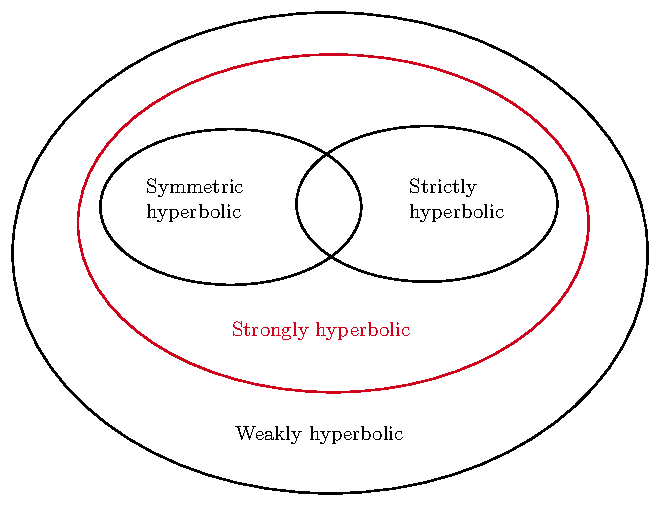
\includegraphics[width=0.5\textwidth]{tikz/weak-hyperbolic.pdf}
    \caption{双曲型问题几个定义之间的关系} \label{fig:weak-hyperbolic}
\end{figure}


\begin{theorem}\label{thm:well-posed-2}
    问题~\eqref{eq:1d-pdes-hyperbolic} 适定的充要条件为:PDEs 为强双曲问题。(弱双曲无法保证适定性)
\end{theorem}

\begin{proof}
    证明见下文。
\end{proof}

考虑带非导数项的问题
\begin{equation}
    \left\{
    \begin{aligned}
         & U_t = A\,U_x  + B\,U \\
         & U(x,0) = F(x)
    \end{aligned}
    \right.
    \label{eq:1d-pdes-hyperbolic-2}
\end{equation}

\begin{theorem}\label{thm:well-posed-3}
    问题~\eqref{eq:1d-pdes-hyperbolic-2} 适定的一个充分条件为:$U_t = A\,U_x$ 为强双曲问题。
\end{theorem}

\begin{proof}
    证明见下文。
\end{proof}

\subsection{抛物型方程组}


考虑一维常系数二阶方程组:周期函数 $U: \mathbb{R} \times \mathbb{R}^+ \to \mathbb{C}^{m}$,常系数矩阵 $A,B,C \in \mathbb{C}^{m \times m}$,满足的 PDEs 为
\begin{equation}
    \left\{
    \begin{aligned}
         & U_t = A\,u_{xx} + B\,U_x + C\,U =: P\,U \\
         & U(x,0) = F(x)
    \end{aligned}
    \right.
    \label{eq:1d-pdes-parabolic}
\end{equation}

\begin{definition}
    称方程组~\eqref{eq:1d-pdes-parabolic} 是抛物型的,如果存在常数 $\delta > 0$,使得 $A$ 的所有特征值 $\lambda$ 都满足 $\Re\, \lambda \ge \delta$。
\end{definition}


\begin{theorem}\label{thm:well-posed-4}
    抛物型问题是适定的。
\end{theorem}

\begin{proof}
    证明见下文。
\end{proof}

\section{一般常系数方程组的适定性}

考虑一般的问题:周期函数 $u: \mathbb{R}^d  \times \mathbb{R}^+ \to \mathbb{C}^{m}$,满足的 PDEs 为
\begin{equation}
    \left\{
    \begin{aligned}
         & u_t = P(\frac{\partial}{\partial x}) u \\
         & u(x,0) = f(x)
    \end{aligned}
    \right.
    \label{eq:pdes-general}
\end{equation}
这里的 $x \in \mathbb{R}^d$ 有多个分量,对应的 $\frac{\partial}{\partial x}$ 是在多重指标意义下的。
谐波解形如
\[
    \widehat{U}(\omega ,t) = e^{\widehat{P}(i \omega )t} \widehat{F}(\omega )
\]

\begin{remark}
    这里的记号 $e^M$ 是矩阵指数
    \[
        e^M = I + M + \frac{M^2}{2!} + \frac{M^3}{3!} + \cdots
    \]
\end{remark}

由于适定性要求对任意初值都成立,可以自然得到如下充要条件:
\begin{theorem}
    初值问题~\eqref{eq:pdes-general} 是适定的,等价于存在常数 $K,\alpha$,使得对于任意 $\omega $ 都有
    \[
        \| e^{\widehat{P}(i \omega )t} \| \le K e^{\alpha t}
    \]
\end{theorem}

这个充要条件不太实用,但是可以据此推出更好用必要或充分条件。
\begin{theorem}[The Petrovskii condition]
    初值问题~\eqref{eq:pdes-general} 适定的必要条件为:存在常数 $\alpha$,使得对于任意 $\omega $,$\widehat{P}(i \omega)$ 的任意特征值 $\lambda(\omega )$,都有
    \[
        \Re\, \lambda(\omega ) \le \alpha
    \]
\end{theorem}

\begin{proof}
    取 $\widehat{P}(i \omega)$ 的任意特征值 $\lambda(\omega )$ 以及对应的单位特征向量 $\phi(\omega )$,满足
    \[
        \widehat{P}(i \omega) \phi(\omega ) = \lambda(\omega ) \phi(\omega ),\quad \Rightarrow \quad e^{\widehat{P}(i \omega)t} \phi(\omega ) = e^{\lambda(\omega )t} \phi(\omega )
    \]
    利用适定性的充要条件可得
    \[
        \left\|e^{\lambda(\omega )t}\right\|  = \left\|e^{\lambda(\omega )t} \phi(\omega ) \right\|
        = \left\| e^{\widehat{P}(i \omega)t} \phi(\omega )\right\| \le K e^{\alpha t}
    \]
    这表明 $\left\|e^{\lambda(\omega )t}\right\|$ 的增长被控制,即实部 $\Re\, \lambda(\omega )$ 存在一致的上界。
\end{proof}

\begin{theorem}\label{thm:well-posed-5}
    初值问题~\eqref{eq:pdes-general} 适定的一个充分条件为:$\widehat{P}(i \omega)$ 始终可以相似对角化,记作
    \[
        \widehat{P}(i \omega) = S(\omega ) \Lambda(\omega ) S^{-1}(\omega ),\quad \forall\,\omega
    \]
    并且满足:
    \begin{enumerate}
        \item 对于相似对角化的变换矩阵 $S(\omega )$,存在与 $\omega $ 无关的常数 $K$,使得
              \[
                  \| S(\omega ) \| \| S^{-1}(\omega ) \| \le K,\quad \forall\,\omega
              \]
        \item (The Petrovskii condition)对于对角阵 $\Lambda(\omega )$,存在与 $\omega $ 无关的常数 $\alpha$,使得
              \[
                  \Re \,\Lambda(\omega ) \le \alpha I,\quad \forall\,\omega
              \]
    \end{enumerate}
\end{theorem}

\begin{proof}
    \[
        \left\| e^{\widehat{P}(i \omega )t} \right\| = \left\| e^{S(\omega ) \Lambda(\omega ) S^{-1}(\omega )t} \right\|
        =
        \left\|S(\omega ) e^{\Lambda(\omega ) t}S^{-1}(\omega ) \right\| \le \left\|S(\omega )\right\| \left\|e^{\Lambda(\omega ) t}\right\| \left\|S^{-1}(\omega ) \right\|
        \le K e^{\alpha t} \qedhere
    \]
\end{proof}


\section{半有界算子与适定性}

仍然考虑的是一般的常系数方程组~\eqref{eq:pdes-general}。

\begin{definition}
    称算子 $P$ 是 $L^2$ 内积意义下的半有界算子,如果 $P$ 满足:存在常数 $\alpha$,使得对任意光滑函数 $v(x)$ 都有
    \[
        (v,Pv)+(Pv,v) \le 2\alpha (v,v)
    \]
    或者等价于要求 $\widehat{P}$ 满足
    \[
        \widehat{P}(i \omega) + \widehat{P}^{\mathsf{H}}(i \omega) \le 2 \alpha I,\quad \forall\,\omega
    \]
\end{definition}

\begin{remark}
    $P$ 是半有界算子并不意味着 $P$ 自身是有界的。
\end{remark}


易知半有界算子可以直接推出问题的适定性:
\begin{theorem}\label{thm:well-posed-6}
    若 $P$ 是 $L^2$ 内积意义下的半有界算子,则问题~\eqref{eq:pdes-general} 是适定的,并且解满足
    \[
        \| u(x,t) \| \le e^{\alpha t} \| u(x,0) \|
    \]
\end{theorem}

\begin{proof}
    \[
        \frac{d}{dt} \left[ e^{-2\alpha  t}(u,u) \right]
        =e^{-2\alpha t}(\frac{d}{dt}(u,u)-2\alpha (u,u))
        = e^{-2 \alpha t}\left[(u ,P u) + (P u,u) - 2\alpha (u,u)\right] \le 0
    \]
    因此
    \begin{gather*}
        e^{-2\alpha t} \| u(x,t) \|^2 \le  \| u(x,0) \|^2 \\
        \| u(x,t) \| \le e^{\alpha t}\| u(x,0) \| \qedhere
    \end{gather*}
\end{proof}

\begin{remark}
    半有界算子只是适定性的充分不必要条件,即使(在当前范数意义下)不是半有界算子,问题也可能是适定的。
\end{remark}

我们还可以通过一个正定矩阵将半有界算子定义中的 $L^2$ 内积和范数进行推广:
考虑一个关于 $\omega $ 的正定矩阵 $\widehat{H}(\omega)$,
此时可以定义一个新的内积 $(\cdot,\cdot)_H$ 和范数 $\| \cdot \|_H$:
\[
    (v_1,v_2)_H := \sum_\omega \langle\hat{v}_1(\omega),\widehat{H}(\omega)\hat{v}_2(\omega)\rangle,\quad
    \| v \|_H := \sqrt{(v,v)_H}
\]
并且要求存在与 $\omega $ 无关的常数 $K>0$ 使得
\[
    \frac{1}{K}I \le \widehat{H}(\omega ) \le K I,\quad \forall\,\omega
\]
这实际是要求新内积和原本的 $L^2$ 内积是等价的。
原本的 $L^2$ 内积相当于选择了平凡的单位阵 $\widehat{H}(\omega ) = I$。

\begin{definition}
    称算子 $P$ 在 $H$ 内积意义下是半有界算子,如果满足存在常数 $\alpha$,使得对任意光滑函数 $v(x)$ 都有
    \[
        (v,Pv)_H + (Pv,v)_H \le 2\alpha (v,v)_H
    \]
    或者等价于要求 $\widehat{P}$ 满足
    \[
        \widehat{H}(\omega ) \widehat{P}(i \omega) + \widehat{P}^{\mathsf{H}}(i \omega) \widehat{H}(\omega ) \le 2\alpha \widehat{H}(\omega ),\quad \forall\,\omega
    \]
\end{definition}
同理可以证明:如果 $P$ 在 $H$ 内积意义下为半有界算子,那么原问题在 $H$ 范数意义下是适定的,
又因为范数等价,在 $L^2$ 范数意义下也是适定的。
利用不同范数意义下的半有界算子,可以得到如下的适定性充要条件:

\begin{theorem}\label{thm:well-posed-7}
    问题~\eqref{eq:pdes-general} 是适定的,等价于可以构造出合适的 $\widehat{H}(\omega )$,使得 $P$ 在 $H$ 内积的意义下为半有界算子,即:存在常数 $K,\alpha >0$,使得
    \begin{gather}
        \frac{1}{K}I \le \widehat{H}(\omega ) \le K I, \quad \forall\,\omega  \label{eq:well-posed-condition-1}\\
        \widehat{H}(\omega ) \widehat{P}(i \omega) + \widehat{P}^{\mathsf{H}}(i \omega) \widehat{H}(\omega ) \le 2\alpha \widehat{H}(\omega ),\quad \forall\,\omega \label{eq:well-posed-condition-2}
    \end{gather}
\end{theorem}


\section{一些定理的证明}

使用半有界算子理论可以简化几个定理的证明过程,因此将证明留在了最后。

\begin{proof}[\normalfont\bfseries Proof of Theorem~\ref{thm:well-posed-2}]
    证明分为如下几个步骤:
    \begin{enumerate}
        \item 首先假设问题~\eqref{eq:1d-pdes-hyperbolic} 是适定的,证明 $A$ 的特征值必须全为实数;
        \item 然后假设 $A$ 的特征值全部为实数,并且具有完备的特征系统,证明问题是适定的;
        \item 最后假设 $A$ 的特征值全部为实数,并且不具备完备的特征系统,证明问题是不适定的。
    \end{enumerate}

    不妨设 $A$ 的特征值为 $\lambda$,对应的特征向量为 $\phi$,满足 $A \phi = \lambda \phi$。
    取初值
    \[
        U(x,0) = e^{i \omega x} \phi.
    \]
    则精确解为
    \[
        U(x,t) = e^{i \omega (x + \lambda t)} \phi.
    \]
    因此
    \[
        \| U(x,t) \| = \| e^{i \omega (x + \lambda t)} \phi \| = e^{\Re(i \omega \lambda t)} \| U(x,0) \|.
    \]
    如果问题是适定的,则存在常数 $\alpha$ 使得
    \[
        \Re(i \omega \lambda t) \le \alpha,\quad \forall\, \omega
    \]
    这表明必然有 $\Im(\lambda) = 0$,即特征值 $\lambda$ 均为实数。

    假设 $A$ 的特征值全部为实数,并且具有完备的特征系统,即 $A$ 可以相似对角化
    \[
        A = S \Lambda S^{-1},\quad \Lambda = \text{diag}(\lambda_1, \cdots, \lambda_m),\quad \lambda_i \in \mathbb{R}.
    \]
    那么通过换元 $U = S V$ 可以得到
    \[
        U_t = A U_x = S \Lambda S^{-1} U_x, \quad \Rightarrow \quad V_t = \Lambda V_x.
    \]
    显然有
    \[
        \| V(x,t) \| = \| V(x,0) \|
    \]
    因此
    \[
        \| U(x,t) \| = \| S\,V(x,t) \| \le \| S \|\,\| V(x,t) \| = \| S \|\,\| V(x,0) \|
        \le  \| S \|\, \| S^{-1} \|\,\| U(x,0) \|
    \]

    最后说明 $A$ 具有完备的特征系统是必要的,通过反证法证明:假设 $A$ 是一个 Jordan 块
    \[
        A = \begin{bmatrix}
            \lambda & 1       &        &         \\
                    & \lambda & \ddots &         \\
                    &         & \ddots & 1       \\
                    &         &        & \lambda \\
        \end{bmatrix}
        = \lambda I + J,\quad \lambda \in \mathbb{R}.
    \]
    取初值
    \[
        U(x,0) = e^{i \omega x} \widehat{U}(\omega,0)
    \]
    则精确解为
    \[
        U(x,t) =  e^{i \omega (\lambda I + J) t} e^{i \omega x} \widehat{U}(\omega,0)
    \]
    因此
    \[
        \|U(x,t)\| \le \|e^{i \omega (\lambda I + J) t}\| \|U(\omega,0)\|
    \]
    问题是适定的等价于存在常数 $K,\alpha$,使得
    \[
        \|e^{i \omega (\lambda I + J) t}\| \le K e^{\alpha t},\quad \forall\,\omega
    \]
    但是注意到
    \[
        \left\| e^{i \omega (\lambda I + J) t} \right\|
        = \left\| e^{i \omega \lambda I t} \right\| \left\| e^{i \omega J t} \right\|
        = \left\| e^{i \omega J t} \right\|
        = \left\|
        \sum_{\ell=0}^{m-1} \frac{(i \omega t)^{\ell}}{\ell!} J^{\ell}
        \right\|
    \]
    显然不存在与 $\omega$ 无关的上界,因此问题不适定。

    综上可得,问题~\eqref{eq:1d-pdes-hyperbolic} 是适定的等价于 $A$ 的特征值全部为实数,并且具有完备的特征系统,即 PDEs 为强双曲问题。
\end{proof}

\begin{proof}[\normalfont\bfseries Proof of Theorem~\ref{thm:well-posed-3}]
    对于 $U_t = A U_x + B U$,由于$A$ 可以相似对角化
    \[
        A = S \Lambda S^{-1},\quad \Lambda = \text{diag}(\lambda_1, \cdots, \lambda_m),\quad \lambda_i \in \mathbb{R}.
    \]
    那么可以通过换元 $U = S V$ 得到
    \[
        U_t = A U_x + B U, \quad \Rightarrow \quad V_t = \Lambda V_x + \widetilde{B} V =: P V.\quad (\widetilde{B} := S^{-1} B S)
    \]
    转换为 Fourier 系数满足的方程组
    \[
        \widehat{V}_t = (i \omega \Lambda + \widetilde{B} S) \widehat{V} =: \widehat{P}(i \omega) \widehat{V}
    \]
    下面证明 $P$ 是半有界算子
    \[
        \widehat{P}(i \omega) + \widehat{P}^\mathsf{H}(i \omega)
        = (i \omega \Lambda + \widetilde{B}) + (- i \omega \Lambda + \widetilde{B}^\mathsf{H})
        = \widetilde{B} + \widetilde{B}^\mathsf{H}
        \le 2 \alpha I,\quad (\alpha = \|\widetilde{B}\|)
    \]
    因此 $V$ 满足
    \[
        \| V(x,t) \| \le e^{\alpha t} \| V(x,0) \|,
    \]
    换元得到 $U$ 满足
    \[
        \| U(x,t) \| = \| S V(x,t) \| \le e^{\alpha t}  \| S \| \| V(x,0) \|
        \le e^{\alpha t}  \| S \| \| S^{-1} \| \| U(x,0) \|
    \]
    因此如果 $U_t = A\,U_x$ 为强双曲问题,则方程~\eqref{eq:1d-pdes-hyperbolic-2} 是适定的。
\end{proof}

为了证明抛物型方程组问题的适定性,我们需要如下引理:
\begin{lemma}\label{lemma:well-posed-1}
    下面两个结论等价:
    \begin{enumerate}
        \item 存在常数 $\delta >0$,使得 $A$ 的所有特征值 $\lambda$ 都满足 $\Re\, \lambda \ge \delta$;
        \item 存在常数 $\delta' >0$ 以及正定矩阵 $H$,使得 $H A + A^{\mathsf{H}} H \ge \delta' H$。
    \end{enumerate}
\end{lemma}

\begin{proof}
    \noindent
    \begin{enumerate}
        \item 假设存在常数 $\delta >0$,使得 $A$ 的所有特征值 $\lambda$ 都满足 $\Re\, \lambda \ge \delta$。
              根据 Schur 引理,可以使用酉方阵 $U$ 将其上三角化
              \[
                  U^\mathsf{H} A U
                  = \begin{bmatrix}
                      \lambda_1 &           &        &        &           \\
                                & \lambda_2 &        &        &           \\
                                &           & \ddots &        &           \\
                                &           &        & \ddots &           \\
                                &           &        &        & \lambda_m
                  \end{bmatrix}
                  +
                  \begin{bmatrix}
                      0 & \tilde{a}_{12} & \cdots         & \cdots & \tilde{a}_{1m}     \\
                        & 0              & \tilde{a}_{23} & \ddots & \tilde{a}_{2m}     \\
                        &                & \ddots         & \ddots & \vdots             \\
                        &                &                & \ddots & \tilde{a}_{m-1\,m} \\
                        &                &                &        & 0
                  \end{bmatrix}
                  =: \Lambda + B
              \]
              定义对角阵 $D_\varepsilon$
              \[
                  D_\varepsilon := \text{diag}(1,\varepsilon,\dots,\varepsilon^{m-1}),\quad (\varepsilon > 0)
              \]
              则有
              \begin{align*}
                  D_\varepsilon^{-1} U^\mathsf{H} A U D_\varepsilon
                  ={} & D_\varepsilon^{-1} ( \Lambda + B ) D_\varepsilon    \\
                  ={} & \begin{bmatrix}
                            \lambda_1 &           &        &        &           \\
                                      & \lambda_2 &        &        &           \\
                                      &           & \ddots &        &           \\
                                      &           &        & \ddots &           \\
                                      &           &        &        & \lambda_m
                        \end{bmatrix}
                  +
                  \begin{bmatrix}
                      0 & \varepsilon \tilde{a}_{12} & \cdots                    & \cdots & \varepsilon^{m-1} \tilde{a}_{1m} \\
                        & 0                          & \varepsilon\tilde{a}_{23} & \ddots & \varepsilon^{m-2} \tilde{a}_{2m} \\
                        &                            & \ddots                    & \ddots & \vdots                           \\
                        &                            &                           & \ddots & \varepsilon \tilde{a}_{m-1\,m}   \\
                        &                            &                           &        & 0
                  \end{bmatrix}
                  \\
                  ={} & \Lambda + D_\varepsilon^{-1} B D_\varepsilon
              \end{align*}
              定义 $\widetilde{A}_\varepsilon = D_\varepsilon^{-1} U^\mathsf{H} A U D_\varepsilon$,显然 $\widetilde{A}_\varepsilon$ 与 $A$ 的特征值相同,并且有
              \[
                  \widetilde{A}_\varepsilon + \widetilde{A}^{\mathsf{H}}_\varepsilon
                  ={}  2 \Re(\Lambda) + D_\varepsilon^{-1} B D_\varepsilon + D_\varepsilon^{\mathsf{H}} B^{\mathsf{H}} D_\varepsilon^{-\mathsf{H}}
                  \ge{}  2 \delta I + D_\varepsilon^{-1} B D_\varepsilon + D_\varepsilon^{\mathsf{H}} B^{\mathsf{H}} D_\varepsilon^{-\mathsf{H}}
              \]
              由于 $\|D_\varepsilon^{-1} B D_\varepsilon\| = \mathcal{O}(\varepsilon)$,
              显然存在 $\varepsilon_0 > 0$,使得当$ 0 < \varepsilon < \varepsilon_0$ 足够小时
              \[
                  \widetilde{A}_\varepsilon + \widetilde{A}^{\mathsf{H}}_\varepsilon \ge \delta I.
              \]
              因此
              \begin{gather*}
                  (U D_\varepsilon)^{-\mathsf{H}} (\widetilde{A}_\varepsilon + A^{\mathsf{H}}_\varepsilon) (U D_\varepsilon)^{-1} \ge \delta\,(U D_\varepsilon)^{-\mathsf{H}} (U D_\varepsilon)^{-1}.
                  \\
                  (U D_\varepsilon)^{-\mathsf{H}} (U D_\varepsilon)^{-1} A + A^{\mathsf{H}} (U D_\varepsilon)^{-\mathsf{H}} (U D_\varepsilon)^{-1} \ge \delta\,(U D_\varepsilon)^{-\mathsf{H}} (U D_\varepsilon)^{-1}.
              \end{gather*}
              取 $H = (U D_\varepsilon)^{-\mathsf{H}} (U D_\varepsilon)^{-1}$ 即可完成证明。
        \item 假设存在常数 $\delta' >0$ 以及正定矩阵 $H$,使得 $H A + A^{\mathsf{H}} H \ge \delta' H$,
              那么对于 $A$ 的任意特征值 $\lambda$ 以及对应的特征向量 $v$,有
              \[
                  0 \le v^{\mathsf{H}} (H A + A^{\mathsf{H}} H - \delta' H) v =  (2 \Re(\lambda) - \delta') v^{\mathsf{H}} H v
              \]
              因此任意特征值均满足 $\Re(\lambda) \ge \frac12\delta'$。
    \end{enumerate}
\end{proof}

\begin{remark}
    上述引理的第一条对应The Petrovskii condition,第二条则对应定理~\ref{thm:well-posed-7} 的条件~\eqref{eq:well-posed-condition-2},
    只是因为二阶导使得不等号全部取反。
\end{remark}

\begin{remark}
    无法通过 $\Re(\lambda(A)) \ge \delta$ 直接推出
    \[
        \exists\,\,\delta' > 0,\quad \text{s.t.} \quad A + A^{\mathsf{H}} \ge \delta' I
    \]
    可以给出一个反例,考虑
    \[
        A = \begin{bmatrix}
            1 & 4 \\
            0 & 1
        \end{bmatrix},\quad  A + A^{\mathsf{H}} = \begin{bmatrix}
            2 & 4 \\
            4 & 2
        \end{bmatrix}
    \]
    $A$ 满足要求,但是 $A + A^{\mathsf{H}}$ 不是正定矩阵。
    但是可以构造合适的 $H$ 满足引理中的要求,例如
    \[
        H = \begin{bmatrix}
            1 & 1 \\
            1 & 6
        \end{bmatrix}, \quad
        H A + A^{\mathsf{H}} H = \begin{bmatrix}
            2 & 6  \\
            6 & 20
        \end{bmatrix} > \frac{1}{10} H
    \]
\end{remark}

\begin{proof}[\normalfont\bfseries Proof of Theorem~\ref{thm:well-posed-4}]
    对于方程组
    \[
        U_t = A U_{xx} + B U_x + C U =: P U
    \]
    转换为 Fourier 系数满足的方程组
    \[
        \widehat{U}_t = (i \omega)^2 A \widehat{U}  + (i \omega) B \widehat{U} + C \widehat{U}
        =: \widehat{P}(i \omega) \widehat{U}
    \]
    由于 PDEs 为抛物型问题,根据引理~\ref{lemma:well-posed-1},存在正定矩阵 $H$ 以及 $\delta > 0$,使得
    \[
        H A + A^\mathsf{H} H \ge \delta H.
    \]
    因此
    \begin{align*}
        H \widehat{P}(i \omega) + \widehat{P}^\mathsf{H}(i \omega) H
        ={}   & \left(-\omega^2 H A + i \omega H B + H C\right)
        + \left(-\omega^2 A^\mathsf{H} H - i \omega B^\mathsf{H} H + C^\mathsf{H} H\right)                \\
        ={}   & -\omega^2 (H A + A^\mathsf{H} H) + i \omega (H B - B^\mathsf{H}H) + (HC + C^\mathsf{H} H) \\
        \le{} & - 2 \delta\, \omega^2 H + i \omega (H B - B^\mathsf{H}H) + (HC + C^\mathsf{H} H)
    \end{align*}
    因为关于 $\omega$ 的二次项系数为负,显然存在与 $\omega$ 无关的有限上界 $\alpha > 0$,使得
    \[
        H \widehat{P}(i \omega) + \widehat{P}^\mathsf{H}(i \omega) H \le 2 \alpha H
    \]
    利用定理~\ref{thm:well-posed-7} 即可证明问题的适定性。
\end{proof}


\section{一些例子}

\begin{example}
    考虑如下偏微分方程组
    \[
        u_t = A u_x + B u,
    \]
    矩阵 $A$, $B$ 在满足何种条件时可以保证能量守恒?(即 $\|u(x,t)\| = \|u(x,0)\|$)
\end{example}

\begin{solution*}
    考虑谐波解
    \[
        u(x,t) = e^{i \omega x} \hat{u}(\omega,t),\quad
        u(x,0) = e^{i \omega x} \hat{f}(\omega)
    \]
    代入方程得到
    \[
        \left\{
        \begin{aligned}
             & \hat{u}_t = (i \omega A + B) \hat{u}, \\
             & \hat{u}(\omega,0) = \hat{f}(\omega)
        \end{aligned}
        \right.
        \quad \Rightarrow \quad
        \hat{u}(\omega,t) = e^{(i \omega A + B)t}\hat{f}(\omega)
    \]
    能量守恒即
    \[
        \| u(x,t) \|^2 =\| u(x,0) \|^2, \quad
        \iff \quad |\hat{u}( \omega,t)|^2 = |\hat{u}( \omega,0)|^2
    \]
    对时间求导
    \begin{align*}
        \partial_t |\hat{u}( \omega,t)|^2
         & = (\hat{u},\hat{u}_t) + (\hat{u}_t,\hat{u})                               \\
         & = (\hat{u},(i \omega A + B) \hat{u}) + ((i \omega A + B) \hat{u},\hat{u}) \\
         & = (\hat{u},(i \omega (A - A^\mathsf{H}) + (B + B^\mathsf{H}))\hat{u})
    \end{align*}
    因此当 $A=A^\mathsf{H}$,$B+B^\mathsf{H}=0$ 时,$\partial_t |\hat{u}( \omega,t)|^2=0$,能量守恒。
\end{solution*}

\begin{example}\label{eg:well-posed-1}
    求证:对于抛物型方程组 $u_t = A u_{xx}$,存在常数 $\delta > 0$ 和 $K > 0$,使得
    \[
        \| u(x,t) \|^2 + \delta \int_0^t \| u_x(x,\xi) \|^2 \,d\xi \le K \| u(x,0) \|^2
    \]
\end{example}

\begin{solution*}
    易知对于抛物方程,存在 $\delta' >0$ 和正定矩阵 $H$ 使得 $H A + A^\mathsf{H} H \ge \delta' H$,
    定义 $H$ 内积以及对应的 $H$ 范数
    \[
        (v_1,v_2)_H := \sum_\omega \langle\hat{v}_1(\omega),H \hat{v}_2(\omega)\rangle
    \]
    显然两个范数是等价的:存在 $C>0$ 使得
    \[
        \frac{1}{C} \| u \|_H^2  \le \| u \|^2 \le C \| u \|_H^2,
    \]

    考虑谐波解
    \[
        u(x,t) = e^{i \omega x} \hat{u}(\omega,t),\quad
        u(x,0) = e^{i \omega x} \hat{f}(\omega)
    \]
    代入方程得到
    \[
        \left\{
        \begin{aligned}
             & \hat{u}_t = (i \omega)^2 A \hat{u}, \\
             & \hat{u}(\omega,0) = \hat{f}(\omega)
        \end{aligned}
        \right.
        \quad \Rightarrow \quad
        \hat{u}(\omega,t) = e^{- \omega^2 A t}\hat{f}(\omega)
    \]
    易得
    \begin{gather*}
        \| u(x,t) \|^2 = \hat{u}^\mathsf{H}(\omega,t) \hat{u}(\omega,t),\quad
        \| u_x(x,t) \|^2 = \omega^2 \hat{u}^\mathsf{H}(\omega,t) \hat{u}(\omega,t), \\
        \| u(x,t) \|_H^2 = \hat{u}^\mathsf{H}(\omega,t) H \hat{u}(\omega,t),\quad
        \| u_x(x,t) \|_H^2 = \omega^2 \hat{u}^\mathsf{H}(\omega,t) H \hat{u}(\omega,t).
    \end{gather*}
    对$\| u(x,t) \|_H^2$关于时间求导
    \begin{align*}
        \partial_t \| u(x,t) \|_H^2
        ={}   & \hat{u}_t^\mathsf{H}(\omega,t) H \hat{u}(\omega,t) + \hat{u}^\mathsf{H}(\omega,t) H \hat{u}_t(\omega,t) \\
        ={}   & - \omega^2 \hat{u}^\mathsf{H}(\omega,t) (A^\mathsf{H} H + H A) \hat{u}(\omega,t)                        \\
        \le{} & - \omega^2 \delta' \hat{u}^\mathsf{H}(\omega,t) H \hat{u}(\omega,t).
    \end{align*}
    因此
    \[
        \partial_t \| u(x,t) \|_H^2 + \omega^2 \delta'\, \hat{u}^\mathsf{H}(\omega,t) H \hat{u}(\omega,t) \le 0
    \]
    对时间积分可得
    \[
        \| u(x,t) \|_H^2  +\omega^2  \delta' \int_0^t \hat{u}^\mathsf{H}(\omega,\xi) H \hat{u}(\omega,\xi) \,d\xi \le \| u(0,t) \|_H^2
    \]
    再利用范数等价性可得
    \[
        \| u(x,t) \|^2  + \delta' \int_0^t \| u_x(x,t) \|^2 \,d\xi \le C^2 \| u(0,t) \|^2
    \]
    取 $K=C^2$,$\delta = \delta'$ 即可得证。
\end{solution*}

\begin{example}
    考虑含低阶项的抛物型方程组
    \[
        u_t = A u_{xx} + B u_x + C u
    \]
    其中 $B$ 是 Hermite 矩阵, $C$ 是反 Hermite 矩阵。
    那么例~\ref{eg:well-posed-1} 中的不等式是否仍然成立?
    \[
        \| u(x,t) \|^2 + \delta \int_0^t \| u_x(x,\xi) \|^2 \,d\xi \le K \| u(x,0) \|^2
    \]
\end{example}

\begin{proof}
    方程 $v_t = A v_{xx}$ 的解 $v$ 满足
    \begin{align*}
        \partial_t \| v(x,t) \|^2
        ={} & \hat{v}_t^\mathsf{H}(\omega,t) \hat{v}(\omega,t) + \hat{v}^\mathsf{H}(\omega,t) \hat{v}_t(\omega,t) \\
        ={} & - \omega^2 \hat{v}^\mathsf{H}(\omega,t) (A^\mathsf{H} + A) \hat{v}(\omega,t).
    \end{align*}
    方程 $u_t = A u_{xx} + B u_x + C u$ 的解 $u$ 满足
    \begin{align*}
        \partial_t \| u(x,t) \|^2
        ={} & \hat{u}_t^\mathsf{H}(\omega,t) \hat{u}(\omega,t) + \hat{u}^\mathsf{H}(\omega,t) \hat{u}_t(\omega,t) \\
        ={} & - \omega^2 \hat{u}^\mathsf{H}(\omega,t) (A^\mathsf{H} + A) \hat{u}(\omega,t)
        - i \omega \hat{u}^\mathsf{H}(\omega,t) (B^\mathsf{H} - B) \hat{u}(\omega,t)                              \\
            & + \hat{u}^\mathsf{H}(\omega,t)(C^\mathsf{H} + C) \hat{u}(\omega,t)                                  \\
        ={} & - \omega^2 \hat{u}^\mathsf{H}(\omega,t) (A^\mathsf{H} + A) \hat{u}(\omega,t).
    \end{align*}
    因此如果对两个方程组选取相同的初值,就有
    \[
        \| u(x,t) \| = \| v(x,t) \|,\quad \forall\, t \ge 0
    \]
    同理
    \[
        \| u_x(x,t) \| = \| v_x(x,t) \|,\quad \forall\, t \ge 0
    \]
    因此原本的估计仍然成立。
\end{proof}

下面提供几个半有界算子的例子。

\begin{example}
    考虑如下偏微分方程组
    \[
        u_t = (A(x,t) u_x)_x =: P u
    \]
    其中矩阵 $A(x,t)$ 关于 $x$ 有周期性,并且满足 $A + A^{\mathsf{H}}$ 的特征值有一致下界 $\delta > 0$,那么 $P$ 是半有界算子。
\end{example}

\begin{proof}
    \begin{align*}
        (u, P u) + (P u, u) ={} & (u, (A u_x)_x) + ((A u_x)_x, u)
        \\
        ={}                     & -(u_x, A u_x) - (A u_x, u_x)    \\
        ={}                     & -(u_x, (A+A^{\mathsf{H}})u_x)   \\
        \le                     & -\delta \, \|u_x\|_2^2 \le 0
    \end{align*}
    取 $\alpha = 0$ 即可满足要求。
\end{proof}

\begin{example}
    考虑如下偏微分方程组
    \[
        u_t = B u_x + C u =: P u
    \]
    其中常系数矩阵 $B,C$,并且 $B$ 是 Hermite 矩阵,那么 $P$ 是半有界算子。
\end{example}

\begin{proof}
    \begin{align*}
        (u, P u) + (P u, u) ={} & (u, B u_x) + (B u_x, u) + (u, C u) + (C u, u)                  \\
        ={}                     & (u, B u_x) -(u, B^{\mathsf{H}} u_x) + (u, (C+C^{\mathsf{H}})u) \\
        ={}                     & (u, (C+C^{\mathsf{H}})u)                                       \\
        \le                     & 2 \| C \| \, \|u\|_2^2
    \end{align*}
    取 $\alpha = \| C \|$ 即可满足要求。
\end{proof}

\begin{example}
    考虑如下偏微分方程组
    \[
        u_t=
        \begin{bmatrix}
            1 & 10 \\
            0 & 2
        \end{bmatrix} u_x.
    \]
    构造合适的 $\widehat{H}(\omega)$,使得 $P$ 在 $H$ 内积意义下为半有界算子,从而利用定理~\ref{thm:well-posed-7} 证明方程组的适定性。
\end{example}

\begin{solution*}
    代入谐波解可以得到
    \[
        \widehat{P}(i\omega)=i\omega \begin{bmatrix}
            1 & 10 \\
            0 & 2
        \end{bmatrix},\quad
        \widehat{P}^\mathsf{H}(i\omega)=-i\omega \begin{bmatrix}
            1  & 0 \\
            10 & 2
        \end{bmatrix}
    \]
    假设 Hermite 矩阵 $\widehat{H}(\omega) = \widehat{H}$ 与 $\omega$ 无关,形如
    \[
        \widehat{H}(\omega)=\begin{bmatrix}
            a       & c \\
            \bar{c} & b
        \end{bmatrix}
    \]
    其中常数 $a,b \in \mathbb{R}$,$c \in \mathbb{C}$。
    此时条件~\eqref{eq:well-posed-condition-1} 等价于要求 $\widehat{H}$ 正定,即两个特征值严格大于0,具体即
    \[
        a > 0,\quad b > 0,\quad a b > |c|^2
    \]
    接下来处理条件~\eqref{eq:well-posed-condition-2}
    \begin{gather*}
        \widehat{H}(\omega)\widehat{P}(i\omega)+\widehat{P}^\mathsf{H}(i\omega)\widehat{H}=
        i\omega \begin{bmatrix}
            0            & 10a+c         \\
            -10a-\bar{c} & 10(\bar{c}-c)
        \end{bmatrix} \\
        2 \alpha \widehat{H} - \left[\widehat{H}(\omega)\widehat{P}(i\omega)+\widehat{P}^\mathsf{H}(i\omega)\widehat{H}\right]
        = \begin{bmatrix}
            2 \alpha a                                   & 2 \alpha c - i \omega(10 a + c)     \\
            2 \alpha \bar{c} + i \omega (10 a + \bar{c}) & 2 \alpha b + i \omega (c - \bar{c})
        \end{bmatrix} =: A
    \end{gather*}
    因此条件~\eqref{eq:well-posed-condition-2} 要求上述矩阵 $A$ 半正定,这等价于要求 $2 \alpha a \ge 0$ 以及
    \[
        \text{det}(A) = 2 \alpha a(2 \alpha b + 10 i \omega(c - \bar{c}))
        - |2\alpha c - i \omega(10a + c)|^2 \ge 0,\quad \forall \omega
    \]
    这个式子是关于 $\omega$ 的实值二次函数,并且二次项系数非正,因此 $\text{det}(A) \ge 0$ 恒成立要求二次项系数严格为0,即
    \[
        10 a + c = 0, \quad \Rightarrow \quad c = -10 a \in \mathbb{R}
    \]
    此时条件变为$\text{det}(A) = 4 \alpha^2 (a b - c^2) \ge 0$,在 $ab > |c|^2$ 时自动成立。


    整理上述所有条件可得
    \[
        a > 0,\quad c = -10 a,\quad b > 100 a.
    \]
    例如可以取 $a=1$,$c = -10$,$b = 200$,构造$\widehat{H}(\omega)=\widehat{H}$为
    \[
        \widehat{H}(\omega)=\widehat{H}=\begin{bmatrix}
            1   & -10 \\
            -10 & 200
        \end{bmatrix}
    \]
    取 $\alpha = 0$ 即可满足~\eqref{eq:well-posed-condition-2}。
    条件~\eqref{eq:well-posed-condition-1} 要求存在 $K > 0$ 使得
    \begin{align*}
        \widehat{H}(\omega)-K^{-1}I & =
        \begin{bmatrix}
            a - \frac{1}{K} & c              \\
            \bar{c}         & b -\frac{1}{K}
        \end{bmatrix}
        =
        \begin{bmatrix}
            1 - \frac{1}{K} & -10              \\
            -10             & 200 -\frac{1}{K}
        \end{bmatrix}
        \ge 0
        \\
        K I-\widehat{H}(\omega)     & =
        \begin{bmatrix}
            K - a    & -c  \\
            -\bar{c} & K-b
        \end{bmatrix}
        =
        \begin{bmatrix}
            K - 1 & 10    \\
            10    & K-200
        \end{bmatrix}
        \ge 0
    \end{align*}
    取足够大的$K$即可满足,例如$K=201$。
\end{solution*}

\begin{remark}
    直接计算 $\widehat{P}(i\omega) + \widehat{P}^\mathsf{H} (i\omega)$ 可得
    \[
        \widehat{P}(i\omega) + \widehat{P}^\mathsf{H} (i\omega) = i \omega
        \begin{bmatrix}
            0 & 10 \\ -10 & 0
        \end{bmatrix}
        =
        \left(\frac{1}{\sqrt{2}}
        \begin{bmatrix}
            -i & i \\ 1 & 1
        \end{bmatrix}\right)
        \begin{bmatrix}
            -10 \omega & \\  & 10 \omega
        \end{bmatrix}
        \left(
        \frac{1}{\sqrt{2}}
        \begin{bmatrix}
            -i & i \\ 1 & 1
        \end{bmatrix}
        \right)^\mathsf{H}
    \]
    因此不存在常数 $\alpha \in \mathbb{R}$ 使得下式成立
    \[
        \widehat{P}(i \omega) + \widehat{P}^\mathsf{H} (i \omega) \le 2\alpha I
    \]
    这表明在 $L^2$ 内积意义下,$P$ 不是半有界算子,不能直接利用定理~\ref{thm:well-posed-6} 证明适定性,
    这同时也表明定理~\ref{thm:well-posed-6} 是适定性的充分不必要条件。
\end{remark}

\begin{remark}
    还可以利用定理~\ref{thm:well-posed-5} 证明该问题的适定性:计算可得 $\widehat{P}(i\omega)$ 的特征值为 $\lambda_1 = i \omega$,$\lambda_2 = 2 i \omega$,始终可以相似对角化
    \[
        \widehat{P}(i\omega) = i \omega
        \begin{bmatrix}
            1 & 10 \\ 0 & 2
        \end{bmatrix}
        =
        \begin{bmatrix}
            10 & 1 \\ 1 & 0
        \end{bmatrix}
        \begin{bmatrix}
            2 i \omega & \\ &  i \omega
        \end{bmatrix}
        \begin{bmatrix}
            10 & 1 \\ 1 & 0
        \end{bmatrix}^{-1}
        = S(\omega) \Lambda(\omega) S(\omega)^{-1}
    \]
    由于 $S(\omega)$ 与 $\omega$ 无关,显然存在常数 $K$ 使得 $\| S(\omega) \| \| S^{-1}(\omega) \| \le K$。
    由于特征值全部为纯虚数,$\Re \Lambda(\omega) = 0$ 满足 The Petrovskii condition。
    定理~\ref{thm:well-posed-5} 的三个条件全部满足,因此该问题是适定的。
\end{remark}
